\chapter{Background Study}
\label{chap:2}

This chapter contains background information on the software, services and algorithms used
in this project. They are divided up into Quick Response Codes (QR Codes), Near Field
Communication (NFC), the web server and the encryption and encoding algorithms used.

\section{Quick Response Codes}

QR Codes are two dimensional bar codes that were initially
 used in Japanese car factories to allow computers to track the progress of
 an item on a production line [\cite{journal:qr-code}]. The technology has
 since evolved and matured and is today widely used in the media industry for storing
 data, such as a web address or a phone number. See Fig. \ref{qrcode} for an example of
 a QR code.
 
\begin{figure}
\centering
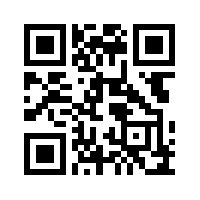
\includegraphics[clip = true, trim = 0 20 0 20, scale = 0.4]{qrcode_voorbeeld.png}
\caption{Example of a QR Code.}
\label{qrcode}
\end{figure}
 
 QR Codes can store up to 7089 alphanumeric characters [\cite{journal:qr-code}], which are
 accessible by scanning the code with either a laser or a digital camera.
 Scanning a QR Code requires a camera that can produce a digital image at a
 resolution that is at least twice that of the QR Code.
 This image is then processed by a QR Code library, e.g.
 the ZXing library (see Sec. \ref{sec:zbar} for more detail on the ZXing library),
 which decodes the picture and extracts the data embedded inside the code. Cellphones are
 commonly used today because of their portability, increasingly powerful hardware and QR
 Code technology's simplicity.
 However, an image with an embedded QR Code can be decoded by any computer with the
 necessary hardware and libraries installed, e.g. a webcam and the ZXing
 library.

\subsection{Zebra Crossing Library}
\label{sec:zbar}

The Zebra Crossing Library (ZXing) is a QR Code coding and decoding
library [\cite{website:zxing}]. It is commonly built into smartphone
applications to decode QR Codes embedded inside a static image or a video
stream. A desktop version of the library, called ZBar, is also available and
works in a similar manner.

The Barcode Scanner application is made by the team that made the ZXing
library. It is freely available on multiple cellphone platforms, such as
BlackBerry OS, Apples's iOS and Google's Android. There have been at least 50 million
downloads of the Barcode Scanner application on the Android platform alone, and it
currently lies 98$^{\rm th}$ in the top 100 of Google Play's most downloaded list
[\cite{website:barcodescanner}]. This shows the extent to which QR Code technology and
the ZXing library has evolved to be used by millions of people.

\section{Near Field Communication}

NFC is a relatively new communication standard in the world of
wireless technology. It allows two NFC-enabled devices to wirelessly transmit data by bringing
them close to one another, typically around 4 centimeters.

Most cellphone manufacturers, with the major exception of Apple, have
added NFC hardware to their flagship models, and more recently to some of
their budget models [\cite{website:nfc-models}]. The technology has also been
ported to other platforms, such as the desktop computer and Arduino. This adds a
new dimension to wireless inter-device communication and makes projects such as
this more feasible.

\subsection{libnfc}

Libnfc is an open-source library for Linux systems [\cite{website:libnfc}]. It allows a
desktop computer to communicate with an NFC device based on the Phillips PN53
series of NFC chips [\cite{website:libnfc-hardware}]. Recent versions have made provision
for the use of a PN532 breakout board that can be used by a Raspberry Pi. It is currently
in version 1.7 and is classified as a `mature' library by the open-source community.

\subsubsection{nfcpy}
\label{sec:nfcpy}

Nfcpy is an open-source Python interface for the libnfc library, developed and maintained
by Stephen Tiedemann [\cite{website:nfcpy}], that allows for peer-to-peer communication
between a cellphone and desktop-based NFC controller. This is done by using the NFC Data
Exchange Format (NDEF), the Simple NDEF Exchange Protocol (SNEP) and the Logical Link Control
Protocol (LLCP). These standards and protocols have been set by the NFC standard governing
body, the NFC Forum [\cite{website:nfc-forum}], to simplify and standardise data exchange
between different platforms, making the user experience more pleasant.

\subsection{Android}

Google's Android operating system (OS) is currently the most popular cellphone OS world
wide, with an estimated 80\% market share [\cite{article:android-marketshare}]. 

Since version 2.3 `Gingerbread', Android has had NFC capabilities
[\cite{website:android-gingerbread}]. Google has since then been promoting the use of NFC
as an alternative payment option. Other platforms, such as Blackberry's OS and Windows Phone, have also added NFC to their latest phones, but they do
not have the market penetration that Android currently has. It was also found that
application development on the Android platform is relatively simple and free. It was
therefore decided that the NFC payment application will be based on the Android platform.

\subsection{RFID and Stellenbosch University Cards}

NFC and Radio Frequency Identification (RFID) technology work in a similar manner: when
two devices  (e.g. cellphone, RFID card, etc.), equipped with an antenna
tuned to a mutual frequency, for example 13.56 MHz, come into close
proximity, they transmit some form of data to one another.

However, there are some important difference between the two technologies. For example, an
NFC system is  an active system, meaning that the device's antenna is always powered. NFC
devices also have peer-to-peer capabilities, meaning that two  devices can communicate
with one another by both sending and receiving data. RFID systems, on the other hand,
only allow for one-way communication [\cite{article:diff-nfc-rfid}] (e.g. the current SU's
student entry control system).

\section{Web Server}

The web server is responsible for handling all the data transfers and transactions that
take place when a customer buys a product. In this section, some background information
will be given on the key features of the web server that was implemented for this project.

\subsection{Django Web Framework}
\label{sec:django}

Django is a Python web server framework which focuses on easy setup and simple design.
Some of its features are that it fully handles Hypertext Transfer Protocol (HTTP)
requests, integrates with SQL databases, supports Hypertext Markup Language (HTML)
template design, makes provision for the execution of Python scripts, and has an offline
server debugging function available. Django is also expandable to commercial size
servers that are accessible across the globe. For example, large websites, such as
Instagram and Pinterest, are based on the Django framework [\cite{website:django-sites}].

To make it easier to program, read and debug, the original Django developers
designed Django to split its websites into multiple, so-called `applications'.
These applications typically contain a single web-page with its own script and
database handling functionality. These applications can communicate with one
another, meaning that a script from application X may execute a script in application Y.

Django was initially developed by web programmers Adrian Holovaty and Simon Willison, from the
newspaper Lawrence Journal World [\cite{website:django-exist}]. It was first released in 2005
under the Berkeley Software Distribution (BSD) license and is completely free to use.

\subsection{Elastic Compute Cloud}
\label{sec:ec2}

Elastic Cloud Compute (EC2) is a cloud computing service offered by Amazon Web
Services (AWS) [\cite{website:aws}]. It allows a user to rent a cloud-based
virtual machine from AWS on which to run their own applications. These applications can be
web-based, which means that these virtual machines are accessible across the world.

\subsection{Apache}
\label{sec:apache}

Apache is a popular web server application (an estimated 53.4\% of the world's servers are
running on it [\cite{website:apache-usage}]) that is available on most OS platforms
[\cite{website:apache-platforms}]. A notable feature of Apache is that it was designed to
be configurable. This makes it easy to run various web frameworks, such as
Python's Django, PHP's cgiapp and C++'s Poco, off of it.

It was initially released by Robert McCool in 1995 under the Apache Licence. It is
currently being maintained by the Apache Software Foundation [\cite{website:apache}].

\section{Encryption}

Encryption is the act of encoding some data into a form that is intended to be
unintelligible to anyone other than the intended recipient.
This is done to ensure that only authorised parties can access sensitive data.
This is often done with an encryption key and an algorithm which
specifies how the data was encrypted and how it can be decrypted. Encryption is often used
where sensitive information is being transmitted between two parties, e.g. personal
e-mails, bank passwords, etc.

Two encryption schemes were considered for this project. They are symmetric
and asymmetric encryption and they are discussed in this section.

\subsection{Symmetric Encryption}

In symmetric encryption, both parties, i.e. the sender and receiver, have to agree to a common
encryption key prior to data transmission [\cite{article:symm-encryption}]. A famous
example of symmetric encryption is the Enigma cipher machine used by Nazi Germany
during the Second World War [\cite{article:enigma}].

Unfortunately, due to the increase in knowledge and understanding around this type of
encryption and the increase in modern computing power, various code cracking
methods, such as known and chosen plain-text attacks 
[\cite{journal:cypher-attacks}] have been developed since 1945 that can break
the most commonly used symmetric encryption methods. However, methods such as
One-Time Pad (OTP) encryption are still being used today. OTP encryption is still
considered to be unbreakable, if done properly [\cite{article:otp}]. However, it is
difficult to securely exchange the keys between the communicating parties
[\cite{article:otp}].

\subsection{Asymmetric Encryption}
\label{sec:assymetric-encryption}

Another encryption scheme is asymmetric encryption, or public-key
encryption. It involves the use of a public and private key pair that can be
used to securely encrypt and sign a data package on the sender's side and to
decrypt and verify the data and its origin on the receiver's side
[\cite{article:pub-encryption}].

These private and public keys are mathematically related to one another
according to the algorithm in use (e.g. ElGamal or RSA. See sections
\ref{sec:elgamal} and \ref{sec:rsa} for more information). The public key is used to
encrypt data and may be publicly distributed. However, in practise the keys are only
distributed to trusted parties to increase security. The private key allows one to
decrypt data encrypted with the public key. 

An advantage of asymmetric encryption is that
even if the public key is leaked, it is still very difficult, and sometimes impossible,
to derive the private key. See Appendix \ref{app:ass-encryption} for a detailed
explanation on asymmetric encryption.

\subsubsection{ElGamal}
\label{sec:elgamal}

The ElGamal algorithm was developed by Taher ElGamal in 1984 [\cite{journal:elgamal}]. It
is an alternative to the popular Ron Rivest, Adi Shamir and Leonard Adleman
(RSA) encryption algorithm. Its security stems from the `difficulty of
computing discrete logarithms in a large prime modulus' [\cite{website:elgamal}].

An advantage that ElGamal has over RSA is that due to the mathematics behind the
algorithm, it is almost certain that a different ciphertext will be generated each time a
string is encrypted. However, a large drawback of this algorithm is that the key
needs to be at least twice as long as the plain-text string that is being encrypted
[\cite{journal:elgamal}].

\subsubsection{RSA}
\label{sec:rsa}

The RSA encryption algorithm is a widely-used encryption standard. Its security is based
on `the difficulty of factoring large integers' [\cite{website:elgamal}]. 

An advantage of the RSA algorithm is its encryption and decryption speed. Also, the
encrypted data's length is determined by the size of the encryption key, provided the
key is long enough. Therefore, the encryptor has some measure of control over how long the
produced ciphertext is going to be.

RSA was developed by Ron Rivest, Adi Shamir and Leonard Adleman in 1978 and has
been widely used since 1993. 

\subsection{PyCrypto}

PyCrypto is a Python cryptography toolkit which contains various encryption algorithms and
key schemes, such as ElGamal, MD5 and RSA. It is currently registered under the
Python License and is available in the public domain. It is maintained by the
PyCrypto Team [\cite{website:pycrypto}].

\subsection{Base64 Encoding}
\label{sec:base64}

Base64 encoding is a scheme which represent arbitrary data as alphanumeric
characters. This encoding scheme is often applied where the output of encrypted
text is a collection of random characters. ASCII characters are normally
preferred because they are easier to read by humans and simpler to transmit via
HTTP. 

Here is an example of a base64 encoded string:\\\\
\textbf{Original text:}\\
Hi, I'm a base64 encoded string!\\
\textbf{Base64 encoded output:}\\
SGksIEknbSBhIGJhc2UgNjQgZW5jb2RlZCBzdHJpbmch
